% vim: set tw=0:
\documentclass{beamer}
\usepackage{graphicx}

% Reasonable themes:
% Antibes Bergen Berkeley Berlin Frankfurt Goettingen Ilmenau Luebeck Malmoe
% Montpellier PaloAlto Rochester Singapore Szeged Warsaw bars boxes
% compatibility default lined plain shadow sidebar split tree
% And these ones include the author's name on every slide:
% Berkeley

% Declare themes.
\mode<presentation>
\usetheme{UWHEP}

% Personal macros.
\newcommand{\email}[1]{{\texttt #1}}
\newcommand{\newframe}[1]{\section{#1}
    \frametitle{\sc{#1}}}
\newcommand{\subframe}[1]{\subsection{#1}
    \frametitle{\sc{#1}}}
\newcommand{\supers}[1]{\ensuremath{^\textrm{#1}}}
\newcommand{\subs}[1]{\ensuremath{_\textrm{#1}}}
\newcommand{\ca}{\ensuremath{\sim}}

% Author information.
\title{T2 Status}
\author[Maier, Mohapatra]{
    Will Maier \and Ajit Mohapatra\\ 
    {\tt wcmaier@hep.wisc.edu}\\
    {\tt ajit@hep.wisc.edu}}
\institute[Wisconsin]{University of Wisconsin - High Energy Physics}
\date{2007.11.27}
\logo{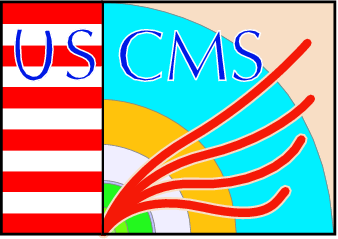
\includegraphics[height=0.6cm]{../../Graphics/USCMS_logo.png}\hspace{.1cm}
\includegraphics[height=0.75cm]{../../Graphics/UW_logo.png}}

\begin{document}

\begin{frame}
    \titlepage
\end{frame}

%\section{Overview}
%\begin{frame}
%    \tableofcontents
%\end{frame}

\section{Facilities}
\subsection{Software and Storage}
\begin{frame}
\frametitle{dCache debugging}
\begin{itemize}
    \item Spontaneous crashes on core dCache machines
    \begin{itemize}
        \item Server hosting GUMS, SRM ran out of memory (will increase on next upgrade)
        \item Unexplained reboots on systems during {\tt cron.daily} (disk I/O?)
    \end{itemize}
    \item Tomcat crashed; no updates to BDII for \ca{}2 weeks
    \begin{itemize}
        \item JVM ran out of memory; applied the session object patch from Ted
    \end{itemize}
    \item Found few corrupted files in dCache
    \begin{itemize}
        \item Scanning pool harddisks and comparing checksums, stat info, etc
        \item Few files have wrong hashes/sizes; most are 'broken' files ('E' in mode, not in PNFS, etc)
    \end{itemize}
    \item Replica Manager over-replicates files
    \begin{itemize}
        \item At worst, we observed \ca{}2.3 replicas per file
        \item RM's reduce function uses odd criteria to decide which files it can reduce
        \item RM continually retries failed reductions
        \item Effectively, no files have been reduced at Wisconsin
    \end{itemize}
\end{itemize}
\end{frame}

\subsection{Production and Monitoring}
\begin{frame}
\frametitle{Newly commissioned link; skims flowing in}
\begin{itemize}
    \item JobRobot: OK
    \item SAM: OK
    \item LoadTest
    \begin{itemize}
        \item Five links commissioned (added CNAF)
        \item Moving skims across all commissioned links to Wisconsin
        \item RAL and PIC are not yet commissioned, so some skims are stuck at PIC
        \item Moving PhEDEx from SL3 to SL4 server (new hardware)
    \end{itemize}
    \item Production
    \begin{itemize}
        \item CSA07 Signal production continues
        \item FNAL, US Tier2s and US Tier3s (Cornell, TTU, FIU-PG) participating
        \item SPRACE not used; UERJ will be back online for production soon
    \end{itemize}
\end{itemize}
\end{frame}

\end{document}
